\documentclass{beamer}
\usepackage[english, russian]{babel}
\usepackage[T2A]{fontenc}
\usepackage[utf8]{inputenc}
\usepackage{indentfirst}
\usepackage{amsmath, amsfonts, amssymb, amsthm, mathtools}
\usepackage[export]{adjustbox}
\usepackage{graphicx} 
\graphicspath{ {./images/} }

\usepackage{subcaption}
\usepackage{verbatim}

\usepackage{minted}{\setlength{\parskip}{0pt}}

\usepackage{hyperref}

\hypersetup{
    colorlinks=true,
    linkcolor=blue,
    filecolor=magenta,      
    urlcolor=black,
    pdftitle={Overleaf Example},
    pdfpagemode=FullScreen,
    }


\title{Отчет по лабораторной работе № 3. \\ Настройка DHCP-сервера}
\author{Данила Стариков \\ НПИбд-02-22}
\date{2024}

\begin{document}

\maketitle
\newpage

\tableofcontents

\newpage
\section{Цель работы}
Приобретение практических навыков по установке и конфигурированию DHCP-сервера.

\newpage
\section{Выполнение работы}

\subsection{Установка DHCP-сервера}
\begin{enumerate}
\item Запустили виртуальную машину server:
    \begin{minted}{bash}
make server-up
    \end{minted}
\item На виртуальной машине server вошли под своим пользователем и открыли терминал. Перешли в режим суперпользователя:
    \begin{minted}{bash}
sudo -i
    \end{minted}
\item Установили dhcp:
    \begin{minted}{bash}
dnf -y install dhcp-server
    \end{minted}
\end{enumerate}

\subsection{Конфигурирование DHCP-сервера}
\begin{enumerate}
    \item Скопировали файл примера конфигурации DHCP dhcpd.conf.example из каталога /usr/share/doc/dhcp* в каталог/etc/dhcp и переименовали его в файл с названием dhcpd.conf (Рис. \ref{01}):
    \begin{minted}{bash}
cd /etc/dhcp
cp /usr/share/doc/dhcp*/dhcpd.conf.example /etc/dhcp
mv /etc/dhcp/dhcpd.conf.example /etc/dhcp/dhcpd.conf
    \end{minted}

\begin{center}
    \centering
    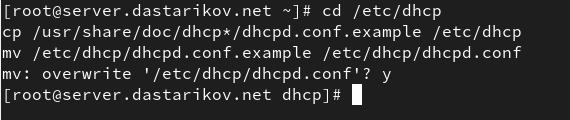
\includegraphics[width=\textwidth]{../images/image01.png}
    \captionof{figure}{Подготовка файла конфигурации.}
    \label{01}
\end{center}

\item Открыли файл /etc/dhcp/dhcpd.conf на редактирование. В этом файле:
    \begin{itemize}
\item Заменили строку
    \begin{minted}{bash}
option domain-name "example.org";
    \end{minted}
на строку
    \begin{minted}{bash}
option domain-name "dastarikov.net";
    \end{minted}
\item Заменили строку
    \begin{minted}{bash}
option domain-name-servers ns1.example.org, ns2.example.org;
    \end{minted}
на строку
    \begin{minted}{bash}
option domain-name-servers ns.dastarikov.net;
    \end{minted}
\item Раскомментировали строку authoritative;
\item На базе одного из приведённых в файле примеров конфигурирования подсети задали собственную конфигурацию dhcp-сети, задав адрес подсети, диапазон адресов для распределения клиентам, адрес маршрутизатора и broadcast-адрес:
    \begin{minted}{bash}
subnet 192.168.1.0 netmask 255.255.255.0 {
range 192.168.1.30 192.168.1.199;
option routers 192.168.1.1;
option broadcast-address 192.168.1.255;
}
    \end{minted}
Остальные примеры задания конфигураций подсетей удалили.
    \end{itemize}
\item Настроили привязку dhcpd к интерфейсу eth1 виртуальной машины server. Для этого скопировали файл dhcpd.service из каталога /lib/systemd/system в каталог /etc/systemd/system (Рис. \ref{02}):
    \begin{minted}{bash}
cp /lib/systemd/system/dhcpd.service /etc/systemd/system/
    \end{minted}
Открыли файл /etc/systemd/system/dhcpd.service на редактирование и заменили в нём строку
    \begin{minted}{bash}
ExecStart=/usr/sbin/dhcpd -f -cf /etc/dhcp/dhcpd.conf -user dhcpd -group dhcpd --no-pid
    \end{minted}
на строку
    \begin{minted}{bash}
ExecStart=/usr/sbin/dhcpd -f -cf /etc/dhcp/dhcpd.conf -user dhcpd -group dhcpd --no-pid eth1
    \end{minted}

\begin{center}
    \centering
    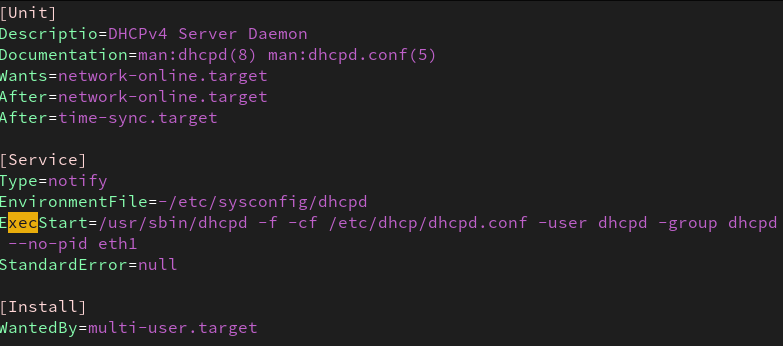
\includegraphics[width=\textwidth]{../images/image02.png}
    \captionof{figure}{Настройка dhcpd.}
    \label{02}
\end{center}

Перезагрузили конфигурацию dhcpd и разрешили загрузку DHCP-сервера при запуске виртуальной машины server (Рис. \ref{03}):
    \begin{minted}{bash}
systemctl --system daemon-reload
systemctl enable dhcpd
    \end{minted}

\begin{center}
    \centering
    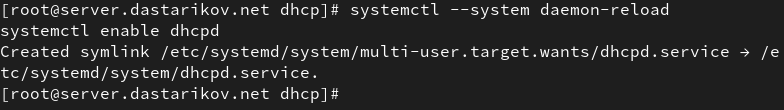
\includegraphics[width=\textwidth]{../images/image03.png}
    \captionof{figure}{Перезагрузка демона dhcpd.}
    \label{03}
\end{center}

\item Добавили запись для DHCP-сервера в конце файла прямой DNS-зоны /var/named/master/fz/dastarikov.net (Рис. \ref{04}):
    \begin{minted}{bash}
dhcp A 192.168.1.1
    \end{minted}

\begin{center}
    \centering
    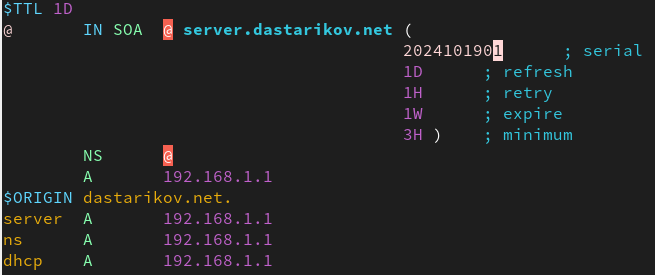
\includegraphics[width=\textwidth]{../images/image04.png}
    \captionof{figure}{Изменение файла прямой DNS-зоны.}
    \label{04}
\end{center}

и в конце файла обратной зоны /var/named/master/rz/192.168.1 (Рис. \ref{05}):
    \begin{minted}{bash}
1 PTR dhcp.dastarikov.net.
    \end{minted}

\begin{center}
    \centering
    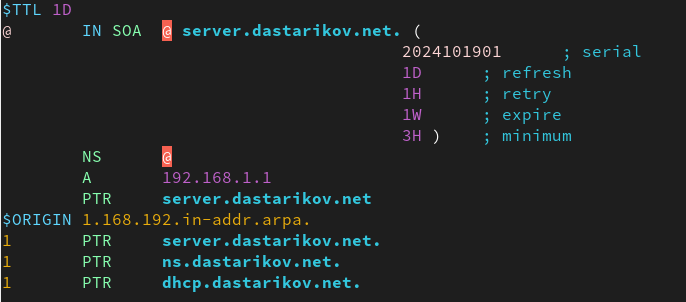
\includegraphics[width=\textwidth]{../images/image05.png}
    \captionof{figure}{Изменение файла обратной DNS-зоны.}
    \label{05}
\end{center}

\item Перезапустили named:
    \begin{minted}{bash}
systemctl restart named
    \end{minted}
\item Проверили, что можно обратиться к DHCP-серверу по имени (Рис. \ref{06}):
    \begin{minted}{bash}
ping dhcp.dastarikov.net
    \end{minted}

\begin{center}
    \centering
    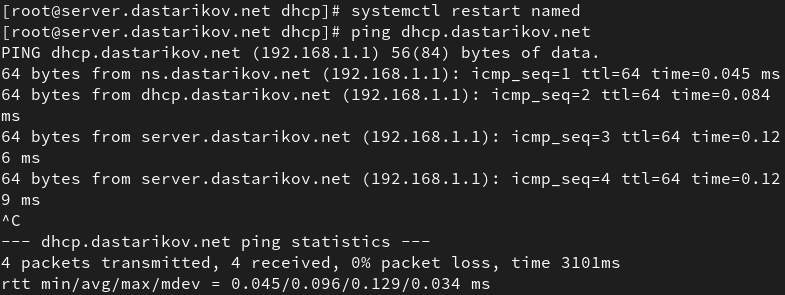
\includegraphics[width=\textwidth]{../images/image06.png}
    \captionof{figure}{Обращение к DHCP-серверу.}
    \label{06}
\end{center}

\item Внесли изменения в настройки межсетевого экрана узла server, разрешив работу с DHCP (Рис. \ref{08}):
    \begin{minted}{bash}
firewall-cmd --list-services
firewall-cmd --get-services
firewall-cmd --add-service=dhcp
firewall-cmd --add-service=dhcp --permanent
    \end{minted}

\begin{center}
    \centering
    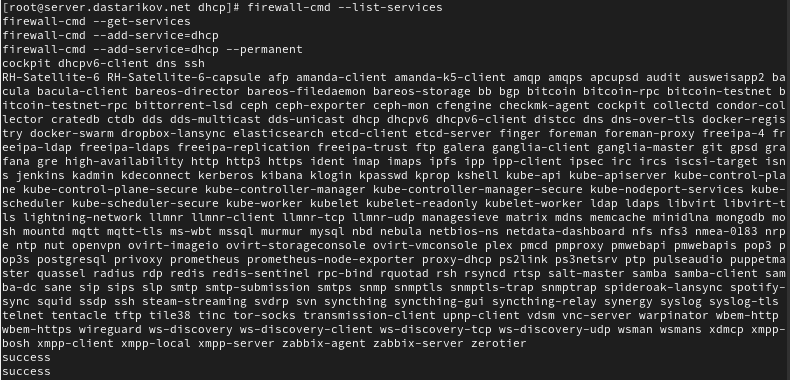
\includegraphics[width=\textwidth]{../images/image08.png}
    \captionof{figure}{Настройка межсетевого экрана для работы с DHCP.}
    \label{08}
\end{center}

\item Восстановили контекст безопасности в SELinux (Рис. \ref{09}):
    \begin{minted}{bash}
restorecon -vR /etc
restorecon -vR /var/named
restorecon -vR /var/lib/dhcpd/
    \end{minted}

\begin{center}
    \centering
    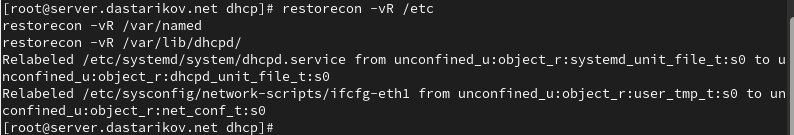
\includegraphics[width=\textwidth]{../images/image09.png}
    \captionof{figure}{Восстановление контекста безопасности SELinux.}
    \label{09}
\end{center}

\item В дополнительном терминале запустили мониторинг происходящих в системе процессов в реальном времени:
    \begin{minted}{bash}
tail -f /var/log/messages
    \end{minted}
\item В основном рабочем терминале запустили DHCP-сервер:
    \begin{minted}{bash}
systemctl start dhcpd
    \end{minted}
\end{enumerate}

\subsection{Анализ работы DHCP-сервера}
\begin{enumerate}
\item Перед запуском виртуальной машины client в каталоге с проектом в основной операционной системе в подкаталоге vagrant/provision/client создали файл 01- routing.sh:
    \begin{minted}{bash}
cd /home/tmp/dastarikov/vagrant/provision/client
touch 01-routing.sh
chmod +x 01-routing.sh
    \end{minted}
Открыв его на редактирование, прописали в нём следующий скрипт:
    \begin{minted}{bash}
#!/bin/bash
echo "Provisioning script $0"
nmcli connection modify "System eth1" ipv4.gateway "192.168.1.1"
nmcli connection up "System eth1"
nmcli connection modify eth0 ipv4.never-default true
nmcli connection modify eth0 ipv6.never-default true
nmcli connection down eth0
nmcli connection up eth0
# systemctl restart NetworkManager
    \end{minted}
Этот скрипт изменяет настройки NetworkManager так, чтобы весь трафик на виртуальной машине client шёл по умолчанию через интерфейс eth1.
\item В Vagrantfile подключили этот скрипт в разделе конфигурации для клиента:
    \begin{minted}{bash}
client.vm.provision "client routing",
type: "shell",
preserve_order: true,
run: "always",
path: "provision/client/01-routing.sh"
    \end{minted}
\item Зафиксировали внесённые изменения для внутренних настроек виртуальной машины client и запустите её, введя в терминале (Рис. \ref{10}):
    \begin{minted}{bash}
make client-provision
    \end{minted}

\begin{center}
    \centering
    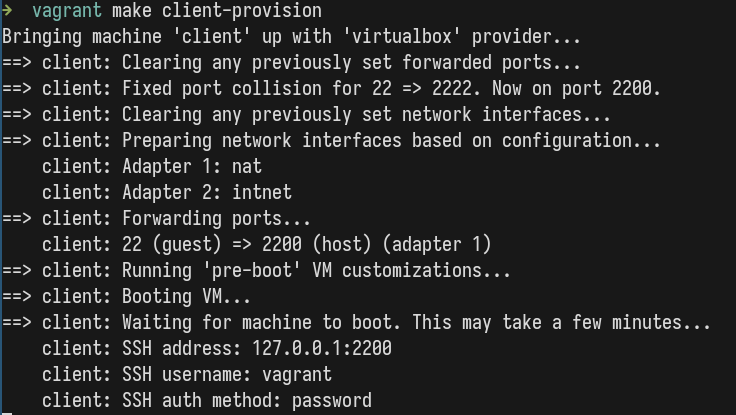
\includegraphics[width=\textwidth]{../images/image10.png}
    \captionof{figure}{Фиксирование внесенных изменений и запуск виртуальной машины client.}
    \label{10}
\end{center}

\item После загрузки виртуальной машины client увидели на виртуальной машине server на терминале с мониторингом происходящих в системе процессов записи о подключении к виртуальной внутренней сети узла client и выдачи ему IP-адреса из соответствующего диапазона адресов. Также информацию о работе DHCP-сервера можно наблюдать в файле /var/lib/dhcpd/dhcpd.leases. В отчёте прокомментируйте построчно информацию из этого файла.
\item Вошли в систему виртуальной машины client под своим пользователем и открыли терминал. В терминале ввели  (Рис. \ref{11})
    \begin{minted}{bash}
ifconfig
    \end{minted}

\begin{center}
    \centering
    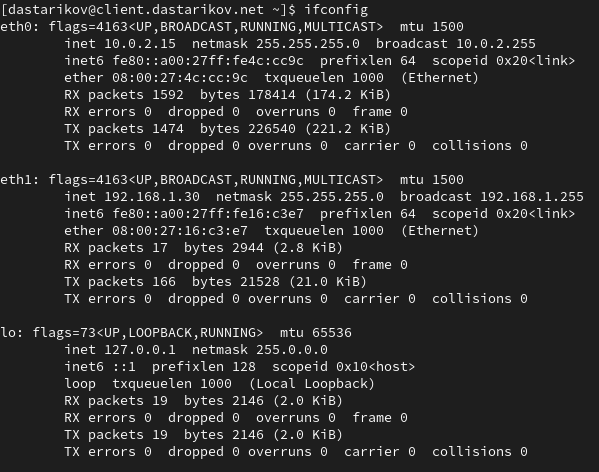
\includegraphics[width=\textwidth]{../images/image11.png}
    \captionof{figure}{Вывод информации об имеющихся интерфейсах.}
    \label{11}
\end{center}

\end{enumerate}

\subsection{Настройка обновления DNS-зоны}
Требуется настроить обновление DNS-зоны при появлении в виртуальной внутренней сети новых узлов.
\begin{enumerate}
\item На виртуальной машине server под пользователем с правами суперпользователя отредактировали файл /etc/named/dastarikov.net, разрешив обновление зоны с локального адреса, т.е. заменив в этом файле в строке allow-update слово none на 127.0.0.1 (Рис. \ref{12}):
    \begin{minted}{bash}
zone "dastarikov.net" IN {
        type master;
        file "master/fz/dastarikov.net";
        allow-update { 127.0.0.1; };
};
zone "1.168.192.in-addr.arpa" IN {
        type master;
        file "master/rz/192.168.1";
        allow-update { 127.0.0.1; };
};
    \end{minted}

\begin{center}
    \centering
    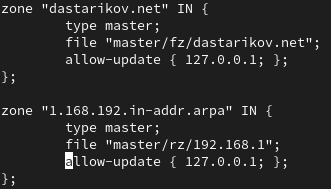
\includegraphics[width=\textwidth]{../images/image12.png}
    \captionof{figure}{Обновление файла DNS-зоны на виртуальной машине server.}
    \label{12}
\end{center}

\item Перезапустили DNS-сервер:
    \begin{minted}{bash}
systemctl restart named
    \end{minted}
\item Внесли изменения в конфигурационный файл /etc/dhcp/dhcpd.conf, добавив в него разрешение на динамическое обновление DNS-записей с локального узла прямой и обратной зон:
    \begin{minted}{bash}
# Use this to enable / disable dynamic dns updates globally.
ddns-updates on;
ddns-update-style interim;
ddns-domainname "dastarikov.net.";
ddns-rev-domainname "in-addr.arpa.";
zone dastarikov.net. {
        primary 127.0.0.1;
}
zone 1.168.192.in-addr.arpa. {
        primary 127.0.0.1;
}
    \end{minted}
\item Перезапустили DHCP-сервер:
    \begin{minted}{bash}
systemctl restart dhcpd
    \end{minted}
\item Если перезапуск DHCP-сервера прошёл успешно, то в каталоге прямой DNS-зоны /var/named/master/fz должен появиться файл dastarikov.net.jnl, в котором в бинарном файле автоматически вносятся изменения записей зоны (Рис. \ref{14}).

\begin{center}
    \centering
    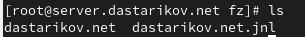
\includegraphics[width=\textwidth]{../images/image14.png}
    \captionof{figure}{Проверка создания файла.}
    \label{14}
\end{center}

\end{enumerate}

\subsection{Внесение изменений в настройки внутреннего окружения
виртуальной машины}
\begin{enumerate}
\item На виртуальной машине server перешли в каталог для внесения изменений в настройки внутреннего окружения /vagrant/provision/server/, создали в нём каталог dhcp, в который поместите в соответствующие подкаталоги конфигурационные файлы DHCP:
    \begin{minted}{bash}
cd /vagrant/provision/server
mkdir -p /vagrant/provision/server/dhcp/etc/dhcp
mkdir -p /vagrant/provision/server/dhcp/etc/systemd/system
cp -R /etc/dhcp/dhcpd.conf /vagrant/provision/server/dhcp/etc/dhcp/
cp -R /etc/systemd/system/dhcpd.service /vagrant/provision/server/dhcp/etc/systemd/system/
    \end{minted}
\item Заменили конфигурационные файлы DNS-сервера:
    \begin{minted}{bash}
cd /vagrant/provision/server/dns/
cp -R /var/named/* /vagrant/provision/server/dns/var/named/
cp -R /etc/named/* /vagrant/provision/server/dns/etc/named/
    \end{minted}
\item В каталоге /vagrant/provision/server создали исполняемый файл dhcp.sh:
    \begin{minted}{bash}
cd /vagrant/provision/server
touch dhcp.sh
chmod +x dhcp.sh
    \end{minted}
Открыв его на редактирование, прописали в нём следующий скрипт:
    \begin{minted}{bash}
#!/bin/bash
echo "Provisioning script $0"
echo "Install needed packages"
dnf -y install dhcp-server
echo "Copy configuration files"
cp -R /vagrant/provision/server/dhcp/etc/* /etc
chown -R dhcpd:dhcpd /etc/dhcp
restorecon -vR /etc
restorecon -vR /var/lib/dhcpd
echo "Configure firewall"
firewall-cmd --add-service=dhcp
firewall-cmd --add-service=dhcp --permanent
echo "Start dhcpd service"
systemctl --system daemon-reload
systemctl enable dhcpd
systemctl start dhcpd
    \end{minted}
\item Для отработки созданного скрипта во время загрузки виртуальной машины server в конфигурационном файле Vagrantfile добавили в разделе конфигурации для сервера:
    \begin{minted}{bash}
server.vm.provision "server dhcp",
type: "shell",
preserve_order: true,
path: "provision/server/dhcp.sh"
    \end{minted}
\item После этого виртуальные машины client и server можно выключить.
\end{enumerate}

\section{Выводы}
В результате выполнения лабораторной работы приобрели практические навыки по установке и конфигурированию DHCP-сервера.

\end{document}
